% answers.tex —— 1994 年·上海卷·数学 · 参考答案与详细解析片段
% 由 tools/generate_projects.py 依来源总账自 1994/1994_数学真题_上海_试题.md + 1994/1994_数学真题_上海_解析正文.md + 1994/1994_数学真题_上海_答案要点.md 生成，勿手改（改源 MD 后重跑）


\begin{gktip}
来源边界：第 1—20 题的下述推导为本项目整理的解答，不是原卷所附印载答案；第 21—26 题据固定来源所附解答整理。整卷尚未经过异人盲核。第 25 题原印载分段条件存在缺区间，保留其文字证据并单独说明复核推导。
\end{gktip}

\begin{answer}
\gksolhead{1}{}

\textbf{题目}：

不等式 $|x+1|<1$ 的解是\gkblank{}。

\Needspace{4\baselineskip}
\textbf{解析}

由 $|x+1|<1$ 得 $-1<x+1<1$，所以 $-2<x<0$。

\gkanswer{答案：$-2<x<0$}

\end{answer}
\begin{answer}
\gksolhead{2}{}

\textbf{题目}：

计算：$\sin\left(\dfrac12\arccos\dfrac18\right)=$\gkblank{}。

\Needspace{4\baselineskip}
\textbf{解析}

\Needspace{5\baselineskip}
设 $\theta=\dfrac12\arccos\dfrac18$。因 $\cos(2\theta)=\dfrac18$ 且 $0<\theta<\dfrac\pi2$，故
\nopagebreak[4]
\[
\sin\theta=\sqrt{\frac{1-\cos(2\theta)}2}=\sqrt{\frac7{16}}=\frac{\sqrt7}{4}\text{。}
\]

\gkanswer{答案：$\dfrac{\sqrt7}{4}$}

\end{answer}
\begin{answer}
\gksolhead{3}{}

\textbf{题目}：

以点 $C(-2,3)$ 为圆心且与 $y$ 轴相切的圆的方程是\gkblank{}。

\Needspace{4\baselineskip}
\textbf{解析}

圆心到 $y$ 轴的距离为 $2$，即半径为 $2$，故圆的方程为 $(x+2)^2+(y-3)^2=4$。

\gkanswer{答案：$(x+2)^2+(y-3)^2=4$}

\end{answer}
\begin{answer}
\gksolhead{4}{}

\textbf{题目}：

方程 $\log_3(x-1)=\log_9(x+5)$ 的解是\gkblank{}。

\Needspace{4\baselineskip}
\textbf{解析}

令 $u=\log_3(x-1)$。因 $\log_9(x+5)=\dfrac12\log_3(x+5)$，原方程等价于 $(x-1)^2=x+5$，并须满足 $x>1$。解得 $x=4$ 或 $x=-1$，仅 $x=4$ 合定义域。

\gkanswer{答案：$x=4$}

\end{answer}
\begin{answer}
\gksolhead{5}{}

\textbf{题目}：

有一个实心圆锥体的零部件，它的轴截面是边长为 $10$ 厘米的等边三角形。现要在它的整个表面镀上一层防腐材料，已知每平方厘米的工料价为 $0.10$ 元，则需要费用\gkblank{}元（$\pi$ 取 $3.2$）。

\Needspace{4\baselineskip}
\textbf{解析}

轴截面为边长 $10$ 的等边三角形，故底半径 $r=5$，母线长 $l=10$。总表面积为 $\pi r^2+\pi rl=25\pi+50\pi=75\pi=240$ 平方厘米（取 $\pi=3.2$），费用为 $240\times0.10=24$ 元。

\gkanswer{答案：$24$ 元}

\end{answer}
\begin{answer}
\gksolhead{6}{}

\textbf{题目}：

函数 $y=\sqrt{x^2-1}\ (x\le -1)$ 的反函数是\gkblank{}。

\Needspace{4\baselineskip}
\textbf{解析}

原函数在 $x\le-1$ 上单调递减且值域为 $[0,+\infty)$。由 $y=\sqrt{x^2-1}$ 得 $x=-\sqrt{y^2+1}$，交换自变量、因变量后，反函数为 $y=-\sqrt{x^2+1}\ (x\ge0)$。

\gkanswer{答案：$y=-\sqrt{x^2+1}\ (x\ge0)$}

\end{answer}
\begin{answer}
\gksolhead{7}{}

\textbf{题目}：

双曲线 $\dfrac{y^2}{2}-x^2=1$ 的两个焦点的坐标是\gkblank{}。

\Needspace{4\baselineskip}
\textbf{解析}

双曲线为 $\dfrac{y^2}{2}-\dfrac{x^2}{1}=1$，故 $a^2=2,b^2=1,c^2=a^2+b^2=3$，焦点为 $(0,\pm\sqrt3)$。

\gkanswer{答案：$(0,\sqrt3)$ 和 $(0,-\sqrt3)$}

\end{answer}
\begin{answer}
\gksolhead{8}{}

\textbf{题目}：

$\left(x^3-\dfrac2{x^2}\right)^5$ 的展开式中 $x^5$ 的系数是\gkblank{}（结果用数值表示）。

\Needspace{4\baselineskip}
\textbf{解析}

通项为 $\binom5k(x^3)^{5-k}(-2x^{-2})^k$，其 $x$ 的次数为 $15-5k$。令 $15-5k=5$ 得 $k=2$，系数为 $\binom52(-2)^2=40$。

\gkanswer{答案：$40$}

\end{answer}
\begin{answer}
\gksolhead{9}{}

\textbf{题目}：

函数 $y=\sin 2x-2\cos^2x$ 的最大值是\gkblank{}。

\Needspace{4\baselineskip}
\textbf{解析}

利用 $2\cos^2x=1+\cos2x$，原式为 $\sin2x-\cos2x-1$。前两项的最大值为 $\sqrt2$，故最大值为 $\sqrt2-1$。

\gkanswer{答案：$\sqrt2-1$}

\end{answer}
\begin{answer}
\gksolhead{10}{}

\textbf{题目}：

\Needspace{5\baselineskip}
函数

\nopagebreak[4]
\[
y=\frac{\sin 2x+\sin\left(2x+\frac\pi3\right)}{\cos 2x+\cos\left(2x+\frac\pi3\right)}
\]

的最小正周期是\gkblank{}。

\Needspace{4\baselineskip}
\textbf{解析}

和差化积后，分子、分母的公因子 $2\cos(\pi/6)$ 约去，得 $y=\tan(2x+\pi/6)$（在原式有定义处）。其最小正周期为 $\pi/2$。

\gkanswer{答案：$\dfrac\pi2$}

\end{answer}
\begin{answer}
\gksolhead{11}{}

\textbf{题目}：

当 $a>1$ 时，函数 $y=\log_a x$ 和 $y=(1-a)x$ 的图象只可能是（　）。
\nopagebreak[4]
\begin{center}% 依固定扫描件第 1 页四种函数图象选项转绘；形态示意，不宣称精确比例。
\begin{center}
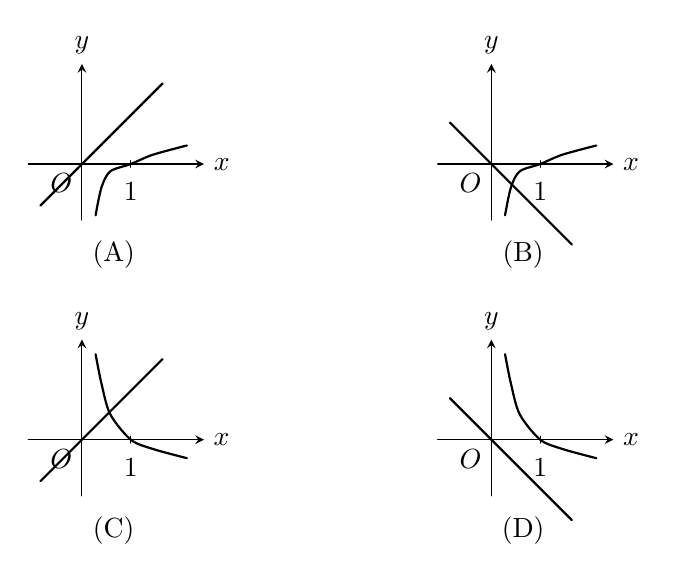
\begin{tikzpicture}[x=0.62cm,y=0.62cm,>=stealth,line cap=round,line join=round]
\foreach \xshift/\yshift/\label/\lineup/\logup in {
  0/3.5/A/1/1, 5.2/3.5/B/-1/1,
  0/0/C/1/-1, 5.2/0/D/-1/-1} {
  \begin{scope}[xshift=\xshift cm,yshift=\yshift cm]
    \draw[->] (-1.1,0)--(2.5,0) node[right] {$x$};
    \draw[->] (0,-1.15)--(0,2.05) node[above] {$y$};
    \draw (1,0.07)--(1,-0.07) node[below=2pt] {$1$};
    \node[below left] at (0,0) {$O$};
    \ifnum\lineup=1
      \draw[thick] (-0.85,-0.85)--(1.65,1.65);
    \else
      \draw[thick] (-0.85,0.85)--(1.65,-1.65);
    \fi
    \ifnum\logup=1
      \draw[thick] plot[smooth] coordinates {(0.28,-1.05) (0.4,-0.48) (0.58,-0.15) (1,0) (1.45,0.19) (2.15,0.38)};
    \else
      \draw[thick] plot[smooth] coordinates {(0.28,1.75) (0.4,1.15) (0.58,0.52) (1,0) (1.45,-0.19) (2.15,-0.38)};
    \fi
    \node[below] at (0.65,-1.38) {(\label)};
  \end{scope}
}
\end{tikzpicture}
\end{center}
\end{center}
\nopagebreak[4]
\Needspace{4\baselineskip}
\textbf{解析}

当 $a>1$ 时，$y=\log_a x$ 在 $x>0$ 上递增、过 $(1,0)$ 且有垂直渐近线 $x=0$；$y=(1-a)x$ 是过原点的负斜率直线。因此只能选 B。

\gkanswer{答案：B}

\end{answer}
\begin{answer}
\gksolhead{12}{}

\textbf{题目}：

如果 $0<a<1$，那么下列不等式中正确的是（　）。

\begin{gkopts}(2)
\task A．$(1-a)^{1/3}>(1-a)^{1/2}$；
\task B．$\log_{1-a}(1+a)>0$；
\task C．$(1-a)^3>(1+a)^2$；
\task D．$(1-a)^{1+a}>1$。
\end{gkopts}

\Needspace{4\baselineskip}
\textbf{解析}

令 $u=1-a\in(0,1)$。指数越大，$u$ 的幂越小，所以 $u^{1/3}>u^{1/2}$，A 正确。$\log_u(1+a)<0$，而 C、D 左边也分别小于右边，故选 A。

\gkanswer{答案：A}

\end{answer}
\begin{answer}
\gksolhead{13}{}

\textbf{题目}：

已知点 $P$ 的极坐标为 $(1,\pi)$，那么过点 $P$ 且垂直于极轴的直线的极坐标方程为（　）。

\begin{gkopts}(1)
\task A．$\rho=1$；B．$\rho=\cos\theta$；C．$\rho=-\dfrac1{\cos\theta}$；D．$\rho=\dfrac1{\cos\theta}$。
\end{gkopts}

\Needspace{4\baselineskip}
\textbf{解析}

点 $P(1,\pi)$ 的直角坐标为 $(-1,0)$。过该点且垂直极轴的直线为 $x=-1$，其极坐标方程 $\rho\cos\theta=-1$，即 $\rho=-1/\cos\theta$，选 C。

\gkanswer{答案：C}

\end{answer}
\begin{answer}
\gksolhead{14}{}

\textbf{题目}：

已知 $a,b$ 是异面直线，直线 $c$ 平行于直线 $a$，那么 $c$ 与 $b$（　）。

\begin{gkopts}(1)
\task A．一定是异面直线；B．一定是相交直线；C．不可能是平行直线；D．不可能是相交直线。
\end{gkopts}

\Needspace{4\baselineskip}
\textbf{解析}

若 $c\parallel b$，因 $c\parallel a$ 将有 $a\parallel b$，与 $a,b$ 异面矛盾，故不可能平行，选 C。$b$ 与 $c$ 是否相交取决于 $c$ 的具体位置，不能断言必相交或必异面。

\gkanswer{答案：C}

\end{answer}
\begin{answer}
\gksolhead{15}{}

\textbf{题目}：

设 $I$ 是全集，集合 $P,Q$ 满足 $P\subset Q$，那么下面的结论中错误的是（　）。

\begin{gkopts}(1)
\task A．$P\cup Q=Q$；B．$\overline P\cup Q=I$；C．$P\cap\overline Q=\varnothing$；D．$\overline P\cap\overline Q=\overline P$。
\end{gkopts}

\Needspace{4\baselineskip}
\textbf{解析}

由 $P\subset Q$ 得前三项分别成立：$P\cup Q=Q$，$\overline P\cup Q=I$，且 $P\cap\overline Q=\varnothing$。又 $\overline Q\subset\overline P$，故 $\overline P\cap\overline Q=\overline Q$，不一定等于 $\overline P$；错误项为 D。

\gkanswer{答案：D}

\end{answer}
\begin{answer}
\gksolhead{16}{}

\textbf{题目}：

设复数 $z=-\dfrac12+\dfrac{\sqrt3}{2}i$（$i$ 为虚数单位），则满足等式 $z^n=z$，且大于 $1$ 的正整数 $n$ 中最小的是（　）。

\begin{gkopts}(2)
\task A．$3$；B．$4$；C．$6$；D．$7$。
\end{gkopts}

\Needspace{4\baselineskip}
\textbf{解析}

$z=\cos\dfrac{2\pi}3+i\sin\dfrac{2\pi}3$。由 $z^n=z$ 得 $n\equiv1\pmod3$，大于 $1$ 的最小正整数是 $4$，选 B。

\gkanswer{答案：B}

\end{answer}
\begin{answer}
\gksolhead{17}{}

\textbf{题目}：

设 $a,b$ 是平面 $\alpha$ 外的任意两条线段，那么“$a,b$ 的长相等”是“$a,b$ 在平面 $\alpha$ 内的射影长相等”的（　）。

\begin{gkopts}(1)
\task A．非充分条件也非必要条件；B．充分必要条件；C．必要条件而非充分条件；D．充分条件而非必要条件。
\end{gkopts}

\Needspace{4\baselineskip}
\textbf{解析}

线段长度相等不保证其在固定平面内的射影长度相等；反之，射影长度相等也不保证原线段长度相等。因此两命题互不构成充分或必要条件，选 A。

\gkanswer{答案：A}

\end{answer}
\begin{answer}
\gksolhead{18}{}

\textbf{题目}：

计划在某画廊展出 $10$ 幅不同的画，其中 $1$ 幅水彩画、$4$ 幅油画、$5$ 幅国画，排成一行陈列。要求同一品种的画必须连在一起，并且水彩画不放在两端，那么不同陈列方式有（　）。

\begin{gkopts}(1)
\task A．$P_4^4\cdot P_5^5$ 种；B．$P_3^3\cdot P_4^4\cdot P_5^5$ 种；C．$C_3^1\cdot P_4^4\cdot P_5^5$ 种；D．$P_2^2\cdot P_4^4\cdot P_5^5$ 种。
\end{gkopts}

\Needspace{4\baselineskip}
\textbf{解析}

同种画必须构成连续块，水彩画块又只能居中。两端的油画块与国画块有 $2!$ 种次序，各块内部分别有 $4!$、$5!$ 种排列，故共 $2!\cdot4!\cdot5!$ 种，选 D。

\gkanswer{答案：D}

\end{answer}
\begin{answer}
\gksolhead{19}{}

\textbf{题目}：

在直角坐标系 $xOy$ 中，曲线 $C$ 的方程是 $y=\cos x$。现平移坐标系，把原点移到点 $O'\left(\dfrac\pi2,-\dfrac\pi2\right)$，那么在坐标系 $x'O'y'$ 中，曲线 $C$ 的方程是（　）。

\begin{gkopts}(1)
\task A．$y'=\sin x'+\dfrac\pi2$；B．$y'=-\sin x'+\dfrac\pi2$；C．$y'=\sin x'-\dfrac\pi2$；D．$y'=-\sin x'-\dfrac\pi2$。
\end{gkopts}

\Needspace{4\baselineskip}
\textbf{解析}

平移后 $x=x'+\pi/2$、$y=y'-\pi/2$。代入 $y=\cos x$ 得 $y'-\pi/2=\cos(x'+\pi/2)=-\sin x'$，所以 $y'=-\sin x'+\pi/2$，选 B。

\gkanswer{答案：B}

\end{answer}
\begin{answer}
\gksolhead{20}{}

\textbf{题目}：

某个命题与自然数 $n$ 有关。如果当 $n=k\ (k\in\mathbb N)$ 时该命题成立，那么可推得当 $n=k+1$ 时该命题也成立。现已知当 $n=5$ 时该命题不成立，那么可推得（　）。

\begin{gkopts}(1)
\task A．当 $n=6$ 时该命题不成立；B．当 $n=6$ 时该命题成立；C．当 $n=4$ 时该命题不成立；D．当 $n=4$ 时该命题成立。
\end{gkopts}

\Needspace{4\baselineskip}
\textbf{解析}

题设是 $P(k)\Rightarrow P(k+1)$。若 $P(4)$ 成立，则推出 $P(5)$ 成立，与已知矛盾；所以 $P(4)$ 不成立，选 C。

\gkanswer{答案：C}

\end{answer}
\begin{answer}
\gksolhead{21}{}

\textbf{题目}：

（本题满分 $12$ 分）已知 $\sin\alpha=\dfrac35$，$\alpha\in\left(\dfrac\pi2,\pi\right)$，$\operatorname{tg}(\pi-\beta)=\dfrac12$，求 $\operatorname{tg}(\alpha-2\beta)$ 的值。

\Needspace{4\baselineskip}
\textbf{解析}

\textbf{解析（据来源印载解答整理）}

\Needspace{5\baselineskip}
由 $\sin\alpha=3/5$ 且 $\alpha$ 在第二象限，得 $\cos\alpha=-4/5$、$\tan\alpha=-3/4$。又 $\tan(\pi-\beta)=1/2$，故 $\tan\beta=-1/2$，从而 $\tan2\beta=-4/3$。于是
\nopagebreak[4]
\[
\tan(\alpha-2\beta)=\frac{-3/4-(-4/3)}{1+(-3/4)(-4/3)}=\frac7{24}\text{。}
\]

\gkanswer{答案：$\dfrac7{24}$。}

\end{answer}
\begin{answer}
\gksolhead{22}{}

\textbf{题目}：

（本题满分 $12$ 分）设 $w$ 为复数，它的辐角的主值为 $\dfrac{3\pi}4$，且 $\dfrac{(\overline w)^2-4}{w}$ 为实数，求复数 $w$。

\Needspace{4\baselineskip}
\textbf{解析}

\textbf{解析（据来源印载解答整理）}

设 $w=a+bi$。由辐角主值为 $3\pi/4$，有 $b=-a$ 且 $a<0$。将 $w=a(1-i)$ 代入条件并取虚部为零，可得 $a^2=2$；结合 $a<0$，得 $w=-\sqrt2+\sqrt2 i$。

\gkanswer{答案：$w=-\sqrt2+\sqrt2i$。}

\end{answer}
\begin{answer}
\gksolhead{23}{}

\textbf{题目}：

（本题满分 $12$ 分）本题共有 $2$ 个小题，第 $1$ 小题满分 $6$ 分，第 $2$ 小题满分 $6$ 分。

如图，在梯形 $ABCD$ 中，$AD\parallel BC$，$\angle ABC=\dfrac\pi2$，$AB=a$，$AD=3a$，且 $\angle ADC=\arcsin\dfrac{\sqrt5}{5}$。又 $PA\perp$ 平面 $ABCD$，$PA=a$。求：
\nopagebreak[4]
\begin{center}% 依固定扫描件第 2 页转绘梯形与棱锥的拓扑关系；不表示精确比例。
\begin{center}
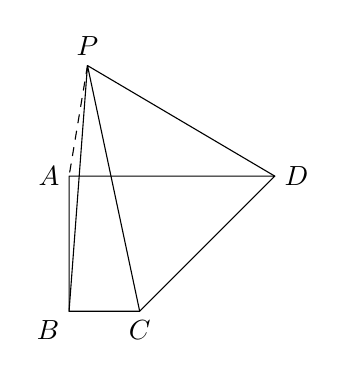
\begin{tikzpicture}[x=0.78cm,y=0.78cm,>=stealth,line cap=round,line join=round]
  \coordinate (B) at (0,0);
  \coordinate (A) at (0,2.2);
  \coordinate (C) at (1.15,0);
  \coordinate (D) at (3.35,2.2);
  \coordinate (P) at (0.3,4.0);
  \draw (A)--(D)--(C)--(B)--cycle;
  \draw (P)--(B) (P)--(C) (P)--(D);
  \draw[dashed] (P)--(A);
  \node[left] at (A) {$A$};
  \node[below left] at (B) {$B$};
  \node[below] at (C) {$C$};
  \node[right] at (D) {$D$};
  \node[above] at (P) {$P$};
\end{tikzpicture}
\end{center}
\end{center}
\nopagebreak[4]
（1） 二面角 $P-CD-A$ 的大小（用反三角函数表示）；

（2） 点 $A$ 到平面 $PBC$ 的距离。

\Needspace{4\baselineskip}
\textbf{解析}

\textbf{解析（据来源印载解答整理）}
\nopagebreak[4]
\begin{center}% 依固定来源解答页转绘辅助点；只表示题目给定线面关系。
\begin{center}
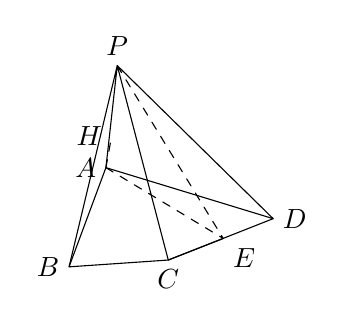
\begin{tikzpicture}[x=0.72cm,y=0.72cm,>=stealth,line cap=round,line join=round]
  \coordinate (B) at (0,0);
  \coordinate (A) at (0.65,1.75);
  \coordinate (C) at (1.75,0.12);
  \coordinate (D) at (3.6,0.85);
  \coordinate (P) at (0.85,3.55);
  \coordinate (E) at (2.72,0.5);
  \coordinate (H) at (0.75,2.3);
  \draw (A)--(D)--(C)--(B)--cycle;
  \draw (P)--(A) (P)--(B) (P)--(C) (P)--(D);
  \draw[dashed] (A)--(E) (P)--(E) (A)--(H);
  \draw (E)--(C);
  \node[left] at (A) {$A$};
  \node[left] at (B) {$B$};
  \node[below] at (C) {$C$};
  \node[right] at (D) {$D$};
  \node[above] at (P) {$P$};
  \node[below right] at (E) {$E$};
  \node[left] at (H) {$H$};
\end{tikzpicture}
\end{center}
\end{center}
\nopagebreak[4]
\textbf{（1）} 在平面 $ABCD$ 内过 $A$ 作 $AE\perp CD$，垂足为 $E$，连接 $PE$。因 $PA\perp$ 平面 $ABCD$，由三垂线定理得 $PE\perp CD$，故 $\angle PEA$ 为所求二面角的平面角。直角三角形 $AED$ 中，$AD=3a$、$\sin\angle ADE=\sqrt5/5$，所以 $AE=3\sqrt5a/5$。再由直角三角形 $PAE$ 得 $\tan\angle PEA=PA/AE=\sqrt5/3$，所求为 $\arctan(\sqrt5/3)$。

\textbf{（2）} 在平面 $PAB$ 内过 $A$ 作 $AH\perp PB$。因 $PA\perp$ 平面 $ABCD$ 且 $AB\perp BC$，得 $BC\perp$ 平面 $PAB$，从而 $AH\perp$ 平面 $PBC$。在等腰直角三角形 $PAB$ 中，$PA=AB=a$，故 $AH=\sqrt2a/2$，即为点 $A$ 到平面 $PBC$ 的距离。

\gkanswer{答案（1）：二面角 $P-CD-A$ 的大小为 $\arctan\dfrac{\sqrt5}{3}$。}

\gkanswer{答案（2）：点 $A$ 到平面 $PBC$ 的距离为 $\dfrac{\sqrt2}{2}a$。}

\end{answer}
\begin{answer}
\gksolhead{24}{}

\textbf{题目}：

（本题满分 $16$ 分）本题共有 $2$ 个小题，第 $1$ 小题满分 $6$ 分，第 $2$ 小题满分 $10$ 分。

设椭圆的中心为原点 $O$，一个焦点为 $F(0,1)$，长轴和短轴的长度之比为 $t$。

（1） 求椭圆的方程；

\Needspace{5\baselineskip}
（2） 设经过原点且斜率为 $t$ 的直线与椭圆在 $y$ 轴右边部分的交点为 $Q$，点 $P$ 在该直线上，且
\nopagebreak[4]
\[
\frac{|OP|}{|OQ|}=t\sqrt{t^2-1}\text{。}
\]
当 $t$ 变化时，求点 $P$ 的轨迹方程，并说明轨迹是什么图形。

\Needspace{4\baselineskip}
\textbf{解析}

\textbf{解析（据来源印载解答整理）}

\Needspace{5\baselineskip}
\textbf{（1）} 设椭圆的长、短半轴分别为 $a,b$。因焦点为 $(0,1)$，有 $a^2-b^2=1$；又 $a/b=t$，解得 $a^2=t^2/(t^2-1)$、$b^2=1/(t^2-1)$。椭圆长轴在 $y$ 轴上，故方程为
\nopagebreak[4]
\[
\frac{x^2}{b^2}+\frac{y^2}{a^2}=1,
\qquad t^2(t^2-1)x^2+(t^2-1)y^2=t^2\text{。}
\]

\textbf{（2）} 在直线 $y=tx$ 上，取椭圆右半平面的交点 $Q$，解得 $Q=(1/\sqrt{2(t^2-1)},\allowbreak\ t/\sqrt{2(t^2-1)})$。距离比给出 $P=\pm t\sqrt{t^2-1}\,Q$，所以 $P=(\pm t/\sqrt2,\ \pm t^2/\sqrt2)$（两坐标同号），消去 $t$ 得两段轨迹：$x^2=\sqrt2y/2$ 且 $x>\sqrt2/2$，以及 $x^2=-\sqrt2y/2$ 且 $x<-\sqrt2/2$。

\gkanswer{答案（1）：$t^2(t^2-1)x^2+(t^2-1)y^2=t^2$。}

\gkanswer{答案（2）：轨迹为抛物线 $x^2=\dfrac{\sqrt2}{2}y$ 在直线 $x=\dfrac{\sqrt2}{2}$ 右侧的部分，以及抛物线 $x^2=-\dfrac{\sqrt2}{2}y$ 在直线 $x=-\dfrac{\sqrt2}{2}$ 左侧的部分。}

\end{answer}
\begin{answer}
\gksolhead{25}{}

\textbf{题目}：

（本题满分 $18$ 分）本题共有 $2$ 个小题，第 $1$ 小题满分 $10$ 分，第 $2$ 小题满分 $8$ 分。

在直角坐标系中，设矩形 $OPQR$ 的顶点按逆时针顺序依次为 $O(0,0)$、$P(1,t)$、$Q(1-2t,2+t)$、$R(-2t,2)$，其中 $t\in(0,+\infty)$。

（1） 求矩形 $OPQR$ 在第一象限部分的面积 $S(t)$；

（2） 确定函数 $S(t)$ 的单调区间，并加以证明。

\Needspace{4\baselineskip}
\textbf{解析}

\textbf{解析；来源印载条件有疑点，以下几何推导待独立复核}

\textbf{（1）} 四边形是平行四边形，因为 $QR=-OP$、$RO=-PQ$。当 $0<t<1/2$ 时，$Q$ 位于第一象限，第一象限部分可由整个平行四边形面积减去两侧不在第一象限的区域求得，化简为 $S(t)=2(1-t+t^2-t^3)$。当 $t\ge1/2$ 时，$Q$ 在 $y$ 轴上或其左侧，第一象限部分是以 $OP$ 为底、与 $y$ 轴交点 $L=(0,t+1/t)$ 为顶点的三角形，故 $S(t)=\dfrac12(t+1/t)$。这支的几何条件是 $t\ge1/2$；固定来源印载解答却写成 $t\ge2$，缺少 $[1/2,2)$，此处保留差异、不得将推导冒充来源原文。
\nopagebreak[4]
\begin{center}% 依固定来源解答页两个情形的矩形与坐标轴示意转绘，不表示精确比例。
\begin{center}
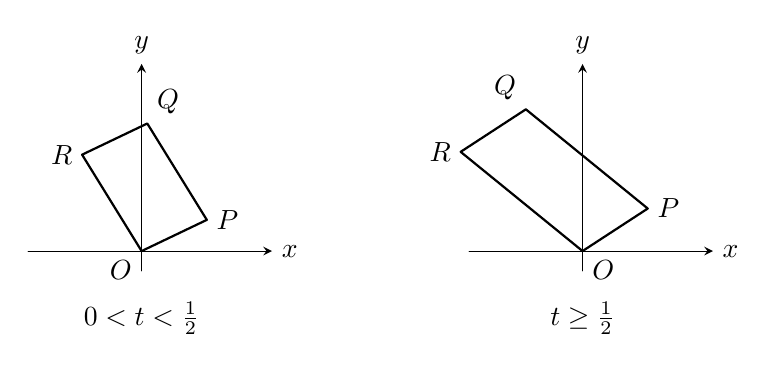
\begin{tikzpicture}[x=0.72cm,y=0.72cm,>=stealth,line cap=round,line join=round]
  \begin{scope}
    \draw[->] (-2,0)--(2.3,0) node[right] {$x$};
    \draw[->] (0,-0.35)--(0,3.3) node[above] {$y$};
    \coordinate (Oa) at (0,0);
    \coordinate (Pa) at (1.15,0.55);
    \coordinate (Qa) at (0.1,2.25);
    \coordinate (Ra) at (-1.05,1.7);
    \draw[thick] (Oa)--(Pa)--(Qa)--(Ra)--cycle;
    \node[below left] at (Oa) {$O$};
    \node[right] at (Pa) {$P$};
    \node[above right] at (Qa) {$Q$};
    \node[left] at (Ra) {$R$};
    \node[below] at (0,-0.72) {$0<t<\frac12$};
  \end{scope}
  \begin{scope}[xshift=5.6cm]
    \draw[->] (-2,0)--(2.3,0) node[right] {$x$};
    \draw[->] (0,-0.35)--(0,3.3) node[above] {$y$};
    \coordinate (Ob) at (0,0);
    \coordinate (Pb) at (1.15,0.75);
    \coordinate (Qb) at (-1.0,2.5);
    \coordinate (Rb) at (-2.15,1.75);
    \draw[thick] (Ob)--(Pb)--(Qb)--(Rb)--cycle;
    \node[below right] at (Ob) {$O$};
    \node[right] at (Pb) {$P$};
    \node[above left] at (Qb) {$Q$};
    \node[left] at (Rb) {$R$};
    \node[below] at (0,-0.72) {$t\ge\frac12$};
  \end{scope}
\end{tikzpicture}
\end{center}
\end{center}
\nopagebreak[4]
\textbf{（2）} 当 $0<t<1/2$ 时，$S'(t)=2(-1+2t-3t^2)<0$。当 $t\ge1/2$ 时，$S'(t)=\dfrac12(1-t^{-2})$，故在 $[1/2,1]$ 上递减，在 $[1,+\infty)$ 上递增。函数在 $t=1/2$ 处连续衔接，因此总体在 $(0,1]$ 上递减、在 $[1,+\infty)$ 上递增。

\gkanswer{答案（1）：$S(t)=\begin{cases}2(1-t+t^2-t^3),&0<t<\dfrac12,\\[3pt]\dfrac12\left(t+\dfrac1t\right),&t\ge2.\end{cases}$}

\gkanswer{答案（2）：见解析版}

\end{answer}
\begin{answer}
\gksolhead{26}{}

\textbf{题目}：

（本题满分 $20$ 分）本题共有 $3$ 个小题，第 $1$ 小题满分 $4$ 分，第 $2$ 小题满分 $8$ 分，第 $3$ 小题满分 $8$ 分。

已知数列 $\{a_n\}$ 满足条件：$a_1=1$，$a_2=r\ (r>0)$，且 $\{a_na_{n+1}\}$ 是公比为 $q\ (q>0)$ 的等比数列。设 $b_n=a_{2n-1}+a_{2n}\ (n=1,2,\ldots)$。

\Needspace{5\baselineskip}
（1） 求出使不等式
\nopagebreak[4]
\[
a_na_{n+1}+a_{n+1}a_{n+2}>a_{n+2}a_{n+3}\quad(n\in\mathbb N)
\]
成立的 $q$ 的取值范围；

（2） 求 $b_n$ 和 $\displaystyle\lim_{n\to\infty}\dfrac1{S_n}$，其中 $S_n=b_1+b_2+\cdots+b_n$；

\Needspace{5\baselineskip}
（3） 设 $r=2^{19.2}-1$，$q=\dfrac12$，求数列
\nopagebreak[4]
\[
\left\{\frac{\log_2 b_{n+1}}{\log_2 b_n}\right\}
\]
的最大项和最小项的值。

\Needspace{4\baselineskip}
\textbf{解析}

\textbf{解析（据来源印载解答整理）}

\textbf{（1）} 令 $c_n=a_na_{n+1}$，则 $c_n=rq^{n-1}$。原不等式等价于 $rq^{n-1}(1+q)>rq^{n+1}$。由 $r,q>0$ 得 $q^2-q-1<0$，所以 $0<q<(1+\sqrt5)/2$。

\textbf{（2）} 由 $a_1a_2=r$ 和公比关系，奇数项、偶数项分别为 $a_{2n-1}=q^{n-1}$、$a_{2n}=rq^{n-1}$，故 $b_n=(1+r)q^{n-1}$。当 $q=1$ 时 $S_n=n(1+r)$，倒数趋于 $0$；当 $0<q<1$ 时 $S_n=(1+r)(1-q^n)/(1-q)$，故极限为 $(1-q)/(1+r)$；当 $q>1$ 时 $S_n$ 趋于无穷，倒数趋于 $0$。

\textbf{（3）} 此时 $b_n=2^{20.2-n}$，令 $c_n=\log_2b_{n+1}/\log_2b_n$，则 $c_n=1+1/(n-20.2)$。对整数 $n\le20$，该式随 $n$ 增大而减小，最小值为 $c_{20}=-4$；对整数 $n\ge21$，该式随 $n$ 增大而减小，最大值为 $c_{21}=9/4$。因此全数列的最大项为 $9/4$，最小项为 $-4$。

\gkanswer{答案（1）：$0<q<\dfrac{1+\sqrt5}{2}$。}

\gkanswer{答案（2）：$b_n=(1+r)q^{n-1}$，且 $\displaystyle\lim_{n\to\infty}\frac1{S_n}=\begin{cases}\dfrac{1-q}{1+r},&0<q<1,\\[3pt]0,&q\ge1.\end{cases}$}

\gkanswer{答案（3）：最大项为 $\dfrac94$，最小项为 $-4$。}

\end{answer}